\section{Gestion de flux de données}\label{sec:rw:supervision:datastream}
Devant la multiplication des applications à base de flux de données telles que : la gestion des données de capteurs ou la surveillance réseau, les \textit{Systèmes de Gestions de Flux de Données} (\textit{SGFD}) ont étés conçus pour mieux maîtriser les données de ce types de systèmes~\cite{Madden:tag, Yao:cougar, Cranor:gigascope}. L'idée principale est de permettre d'utiliser les flux de données de la même manière que les bases de données. L'interrogation des flux passe par un langage déclaratif (tout comme le \textit{SQL}) avec un grand pouvoir d'expression.

La gestion de flux est le socle fondamental des systèmes capables de traiter les événements. Les travaux récents sur les \textit{CEP} (\textit{Complex Event Processing}) permettant de faire de la détection d'événement complexe~\cite{Brenna:cayuga} sont au final une extension des SGFD avec des opérateurs spécifiques et optimisés.
\subsection{Approche des SGFD}
Un flux de données est une série de données qui s'accumule au fur et à mesure du temps~\cite{Golab:issues}. De façon générale, il n'est pas supposé une régularité temporelle sur l'arrivée des données dans le flux (tel que \enquote{\it une donnée toutes les 5 secondes}). L'idée de faire une interrogation sur ces flux de données au sens \enquote{gestion de base de données} du terme n'a pas de sens car il y aurait confusion entre les modes d'interrogations continues et instantanées présentés en section~\ref{sec:intro:problematique}. En effet, le paradigme des requêtes est fondamentalement différent car les requêtes sont de longue durée et persistantes~\cite{Chen:niagaracq} comme illustré dans la figure~\ref{fig:rw:supervision:sgbd-sgfd}.
\begin{figure}[ht]
    \centering
    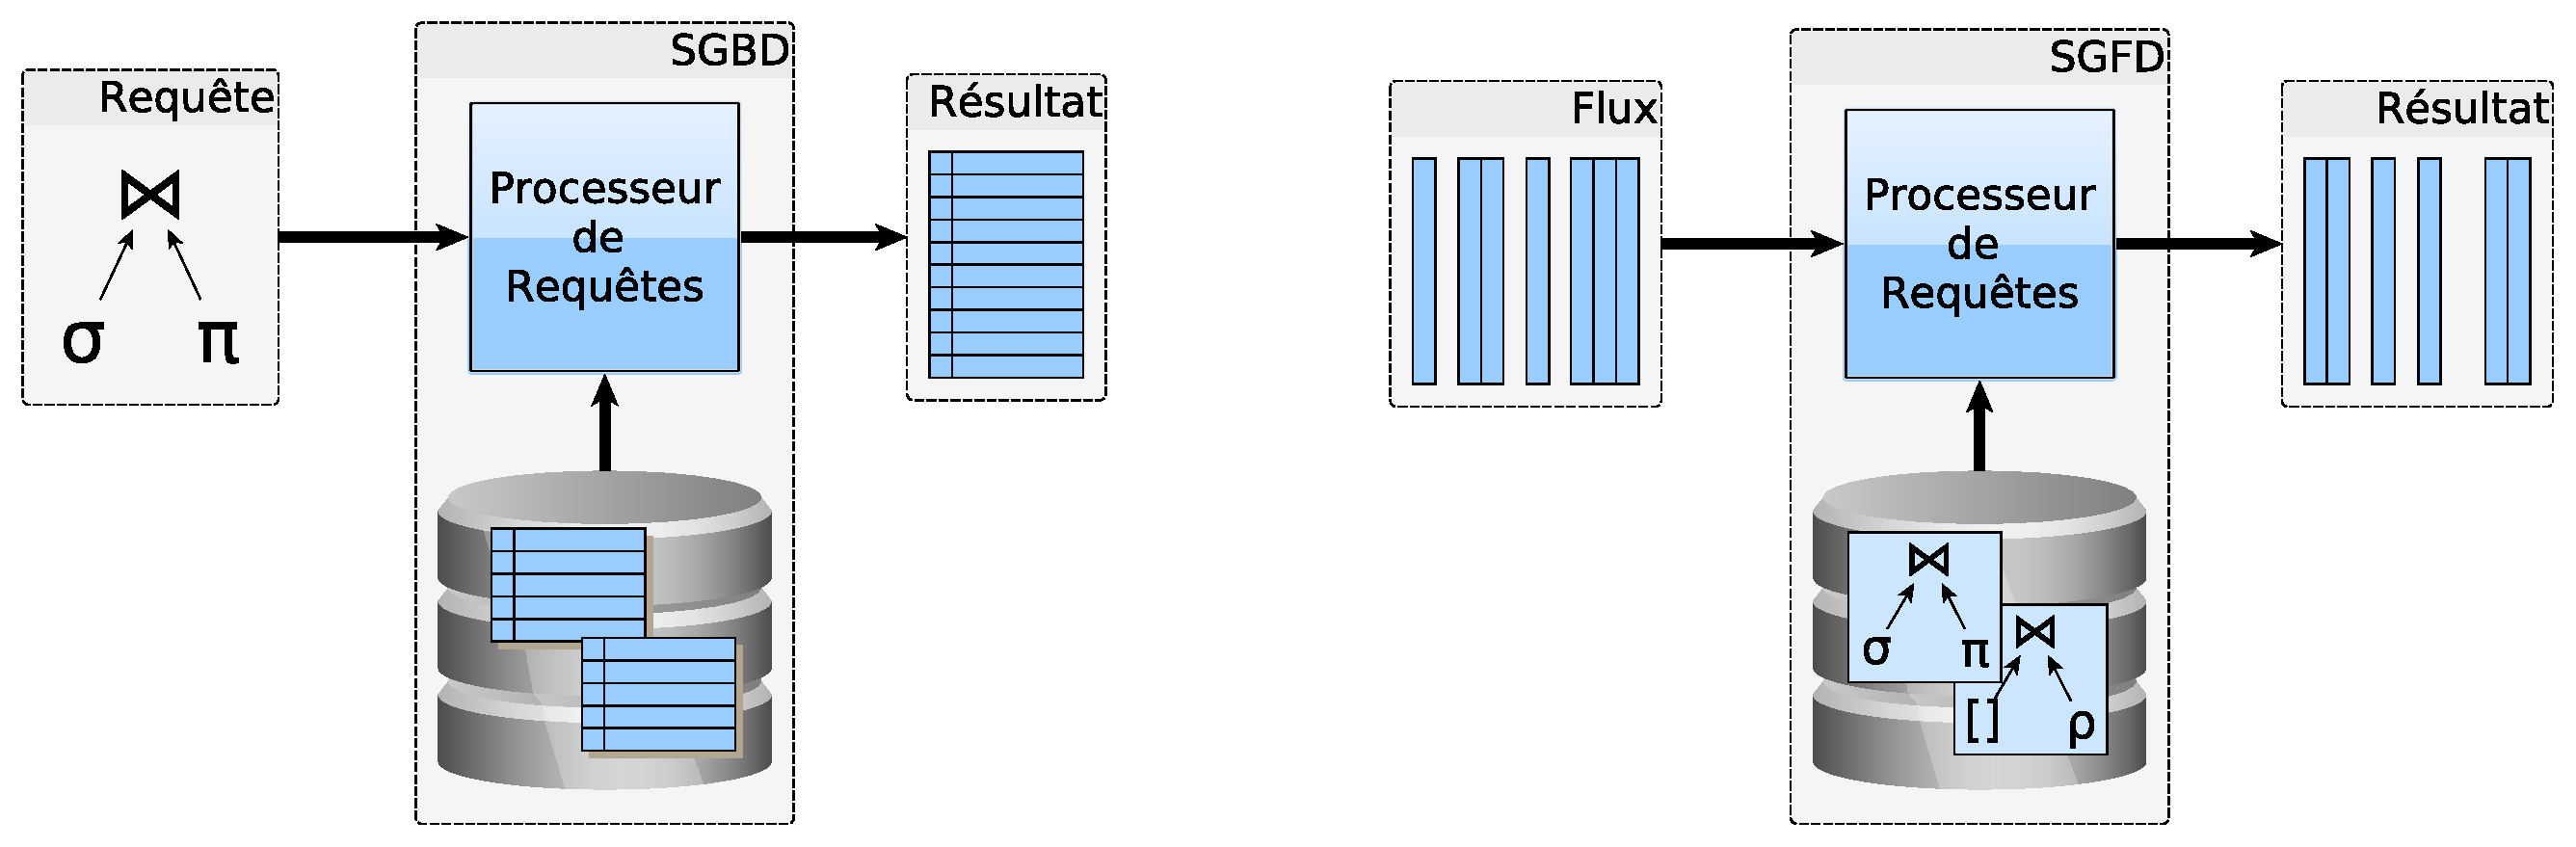
\includegraphics[width=0.75\textwidth]{rw-supervision-sgbd-sgfd}
    \caption{SGBD : Requêtes transitoires, Données persistantes vs SGFD : Données transitoires, Requêtes persistantes~\protect\cite{Gurgen:sstreamware}}\label{fig:rw:supervision:sgbd-sgfd}
\end{figure}

\begin{itemize}
    \item[\textbf{Base de données}] : Une requête est une question posée sur un ensemble de relations figées et persistants (principe transactionnel). La réponse est un ensemble de n-uplets. Une fois la requête traitée elle n'existe plus.
    \item[\textbf{Flux de données}] : Une requête un ensemble d'opérateurs et est considéré comme persistant. Le ou les flux de données sont appliqués sur cet ensemble d'opérateurs pour en produire un nouveau flux. La particularité d'un flux de données est qu'une fois la donnée \textit{consommée}, elle n'est plus considéré comme présente dans le flux d'entrée. Les données fournies en entrée de la requête sont  transitoires.
\end{itemize}

Ainsi, le terme \textit{requête} a un tout autre sens. Toutefois, beaucoup de concepts sont applicables dans ce contexte. En effet, plusieurs éléments du modèle relationnel sont appliqués dans ce domaine~\cite{Arasu:semantic}. Historiquement, les premières requêtes continues~\cite{Terry:tapestry} étaient une exécution périodique de requêtes \textit{SQL}. Le traitement était entièrement basé sur les opérateurs du modèle relationnel standard. Par la suite, les modèles ont évolués pour supporter le dynamisme propre aux flux.

\subsection{Intérêt pour l'observation de systèmes}
La gestion de flux de données a été créée pour mieux gérer le dynamisme des données. Le résultat montre qu'effectivement, il est possible de faire des requêtes continues sur des flux de données de manière déclarative et avec des performances très efficaces. Toutefois, la complexité qui en ressort comparée à celle de l'algèbre relationelle est plus importante. Beaucoup de systèmes n'ayant pas besoin de cette diversité restreignent leurs opérateurs pour être plus facilement utilisable. L'exemple le plus courant est le domaine de la gestion de flux d'actualité (\textit{RSS}) où le schéma est constant et l'intégration à base d'union.

Les données sont toutefois considérées comme uniquement volatiles. Pour notre problématique, il est nécessaire de pouvoir gérer les données persistantes et les requêtes instantanées. Cette approche semble être la plus proche de notre objectif. Ainsi, nous consacrons le chapitre~\ref{chap:rw:sgfd} à son analyse détaillée.

\begin{table}[!ht]
\criteretabDonnee
    {Modèle dérivé du relationnel mais où le contenu est variable dans le temps.}
    {Ensemble de sources indépendantes sauf représentation ad-hoc.}
    {Toutes les données sont dynamiques et événementielles a priori.}
\criteretabTraitement
    {Continue.}
    {Il est supposé que chaque source produit un flux de données. Le fait de traiter ces flux participe à l'intégration de sources.}
    {Langages de requêtes similaires aux SQL supportant la dynamique des données}
    {A un instant donné, les opérateurs sont semblables au relationnel. L'expressivité du support de l'évolution des données reste inconnu encore.}
\criteretabAdaptabilite
    {Création de source pour fournir les flux de données. Comme il n'y a pas de schéma conceptuel, l'adaptation est l'écriture de requêtes continues.}
    {Pas de perspectives métiers.}
    {Les sources et puits sont en général adaptés par les utilisateurs. Un développement peut être fait dessus, mais il est rarement possible de rajouter des opérateurs.}
    {Très rapide car la latence de traitement doit être contrôlée pour supporter des haut débits.}
\caption{Synthèse des systèmes de gestion de flux de données}\label{tab:rw:supervision:sgfd:synthese}
\end{table}
